\chapter{ランサムウェア}
% 本章では,本研究の提案手法に関連する要素に注目して,ランサムウェアについて説明する.





\section{概要}

ランサムウェアとはマルウェアの一種であり,攻撃者が要求した金額が支払われるまで,システムやデータへのアクセスを制限する.
言い換えると,データや計算資源,サービスなどのリソースを人質に取って被害者を脅迫することで身代金を要求するマルウェアがランサムウェアである.

ランサムウェアはリソースへのアクセスを制限する方法に基づいて暗号化ランサムウェアとロッカーランサムウェアに分類される \cite{oz2022survey}.
暗号化ランサムウェアは感染先ホストのファイルやデータを暗号化し,元のファイルを削除または上書きする.
ロッカーランサムウェアは暗号化を行わず,デスクトップのスクリーンやブラウザをロックすることで被害者がシステムを利用できないようにする.
本研究は暗号化ランサムウェアを対象としているため,本稿では暗号化ランサムウェアを単に「ランサムウェア」と呼ぶことにする.

AIDS Trojan \cite{aids-trojan} は1989年に最初のランサムウェアとして登場した.
AIDS Trojanは被害者に郵送されたフロッピーディスクを介して感染し,Windowsシステムを対象としていた.
その後インターネットの普及に伴い,ランサムウェアによる被害が増加し始めた.
2005年に登場したGPCode \cite{PGPCoder42:online} はフィッシングメールを介して感染し,独自の暗号化アルゴリズムによってファイルを暗号化した.

現代のランサムウェアはますます高度化している.
ランサムウェアの進化における重要な要素を以下に列挙する.
\begin{itemize}
  \item AESなどの対称鍵暗号化アルゴリズムやRSA,楕円曲線暗号などの非対称鍵暗号化アルゴリズムを使用して暗号化を行うようになっている \cite{Evolution-Ransomware}.
        これにより,復号鍵を入手することができなければデータの復号はほぼ不可能となった.

  \item Windowsだけでなく,Linux,macOS,Androidなどの他のOSを対象としたランサムウェアも登場するようになった.

  \item ビットコインに代表される仮想通貨が普及したことで身代金の支払いが匿名で行えるようになり,攻撃者の特定が難しくなった.

  \item ランサムウェアの開発と配布を有料で行うサービスであるRansomware as a Service (RaaS) が登場し,専門知識が無くとも容易に攻撃を実施することができるようになった.

  \item 無差別的な攻撃から,特定の高価値な組織 (政府機関や大企業など) を対象とした高度な攻撃に移行しつつある \cite{early-detection}.

\end{itemize}


\section{次}

\subsection{下}

これは,本論の文章である.これは,本論の文章である.
これは,本論の文章である.これは,本論の文章である.
これは,本論の文章である.これは,本論の文章である.
これは,本論の文章である.これは,本論の文章である.
これは,本論の文章である.これは,本論の文章である.

\subsection{その次}

これは,本論の文章である.これは,本論の文章である.

これは,本論の文章である.これは,本論の文章である.
これは,本論の文章である.これは,本論の文章である.
これは,本論の文章である.これは,本論の文章\footnote{
  脚注はこのように書く.}
である.
これは,本論の文章である.これは,本論\footnote{
  脚注を入れすぎると読みにくくなるという意見もある.
  長文の脚注も避けるべきであるとの主張もある.
  適切な脚注になっているかどうか,十分検討すべきである.}
の文章である.

\begin{equation}\label{eq:sample}
  \sum_{k = 1}^{n} = \frac{n(n+1)}{2}
\end{equation}

これは,本論の文章である.これは,本論の文章である.
これは,本論の文章である.これは,本論の文章である.
これは,本論の文章である.これは,本論の文章である.
これは,本論の文章である.これは,本論の文章である.
これは,本論の文章である.これは,本論の文章である.
これは,本論の文章である.これは,本論の文章である.
これは,本論の文章である.これは,本論の文章である.
式(\ref{eq:sample})より,結論が得られる.
詳細は,図\ref{figure:sample}を参照.

\begin{figure}[tbp]
  \begin{center}
    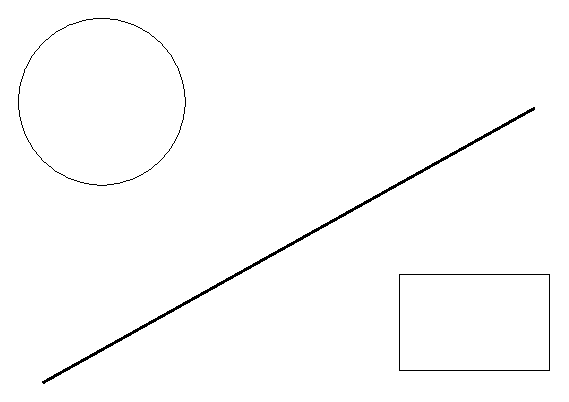
\includegraphics[width=0.5\columnwidth]{fig.eps}
  \end{center}
  \caption{\label{figure:sample}図のタイトル}
\end{figure}

\subsection{そのまた次}

この節は,1ページすべてが文章で埋め尽くされる例を示している.
この節は,1ページすべてが文章で埋め尽くされる例を示している.
この節は,1ページすべてが文章で埋め尽くされる例を示している.
この節は,1ページすべてが文章で埋め尽くされる例を示している.
この節は,1ページすべてが文章で埋め尽くされる例を示している.

この節は,1ページすべてが文章で埋め尽くされる例を示している.
この節は,1ページすべてが文章で埋め尽くされる例を示している.
この節は,1ページすべてが文章で埋め尽くされる例を示している.
この節は,1ページすべてが文章で埋め尽くされる例を示している.
この節は,1ページすべてが文章で埋め尽くされる例を示している.
この節は,1ページすべてが文章で埋め尽くされる例を示している.
この節は,1ページすべてが文章で埋め尽くされる例を示している.
この節は,1ページすべてが文章で埋め尽くされる例を示している.
この節は,1ページすべてが文章で埋め尽くされる例を示している.
この節は,1ページすべてが文章で埋め尽くされる例を示している.

この節は,1ページすべてが文章で埋め尽くされる例を示している.
この節は,1ページすべてが文章で埋め尽くされる例を示している.
この節は,1ページすべてが文章で埋め尽くされる例を示している.
この節は,1ページすべてが文章で埋め尽くされる例を示している.
この節は,1ページすべてが文章で埋め尽くされる例を示している.

この節は,1ページすべてが文章で埋め尽くされる例を示している.
この節は,1ページすべてが文章で埋め尽くされる例を示している.
この節は,1ページすべてが文章で埋め尽くされる例を示している.
この節は,1ページすべてが文章で埋め尽くされる例を示している.
この節は,1ページすべてが文章で埋め尽くされる例を示している.
この節は,1ページすべてが文章で埋め尽くされる例を示している.
この節は,1ページすべてが文章で埋め尽くされる例を示している.
この節は,1ページすべてが文章で埋め尽くされる例を示している.
この節は,1ページすべてが文章で埋め尽くされる例を示している.
この節は,1ページすべてが文章で埋め尽くされる例を示している.

この節は,1ページすべてが文章で埋め尽くされる例を示している.
この節は,1ページすべてが文章で埋め尽くされる例を示している.
この節は,1ページすべてが文章で埋め尽くされる例を示している.
この節は,1ページすべてが文章で埋め尽くされる例を示している.
この節は,1ページすべてが文章で埋め尽くされる例を示している.

この節は,1ページすべてが文章で埋め尽くされる例を示している.
この節は,1ページすべてが文章で埋め尽くされる例を示している.
この節は,1ページすべてが文章で埋め尽くされる例を示している.
この節は,1ページすべてが文章で埋め尽くされる例を示している.
この節は,1ページすべてが文章で埋め尽くされる例を示している.
この節は,1ページすべてが文章で埋め尽くされる例を示している.
この節は,1ページすべてが文章で埋め尽くされる例を示している.
この節は,1ページすべてが文章で埋め尽くされる例を示している.
この節は,1ページすべてが文章で埋め尽くされる例を示している.
この節は,1ページすべてが文章で埋め尽くされる例を示している.

この節は,1ページすべてが文章で埋め尽くされる例を示している.
この節は,1ページすべてが文章で埋め尽くされる例を示している.
この節は,1ページすべてが文章で埋め尽くされる例を示している.
この節は,1ページすべてが文章で埋め尽くされる例を示している.
この節は,1ページすべてが文章で埋め尽くされる例を示している.

この節は,1ページすべてが文章で埋め尽くされる例を示している.
この節は,1ページすべてが文章で埋め尽くされる例を示している.
この節は,1ページすべてが文章で埋め尽くされる例を示している.
この節は,1ページすべてが文章で埋め尽くされる例を示している.
この節は,1ページすべてが文章で埋め尽くされる例を示している.
この節は,1ページすべてが文章で埋め尽くされる例を示している.
この節は,1ページすべてが文章で埋め尽くされる例を示している.
この節は,1ページすべてが文章で埋め尽くされる例を示している.
この節は,1ページすべてが文章で埋め尽くされる例を示している.
この節は,1ページすべてが文章で埋め尽くされる例を示している.

この節は,1ページすべてが文章で埋め尽くされる例を示している.
この節は,1ページすべてが文章で埋め尽くされる例を示している.
この節は,1ページすべてが文章で埋め尽くされる例を示している.
この節は,1ページすべてが文章で埋め尽くされる例を示している.
この節は,1ページすべてが文章で埋め尽くされる例を示している.


\section{最後}

これは,本論の文章である.これは,本論の文章である.
これは,本論の文章である.これは,本論の文章である.
これは,本論の文章である.これは,本論の文章である.

これは,本論の文章である.これは,本論の文章である.
これは,本論の文章である.これは,本論の文章である.
これは,本論の文章である.これは,本論の文章である.

